\documentclass[12pt, logo=tehranDLDL/ut]{tehranDLDL}
\usepackage{subcaption}
\usepackage{pgfplots}
\usepackage{todonotes}
\usepackage{amsmath}
\usepackage{multicol}

\suptitle{Experiment 4}
\supsubtitle{Sessions 9, 10}
\title{Audio Processing}
\author{Katayoon Basharkhah \& Hadi Safari}
\preparer{Katayoon Basharkhah}
\supervisor{Professor Z. Navabi}
\university{University of Tehran}
\college{College of Engineering\\School of Electrical \& Computer Engineering}
\course[DLLab]{Digital Logic Laboratory}
\coursecode{ECE 045}
\courseurl{https://gitlab.com/hadi_sfr/ut-dldlab/-/jobs/artifacts/master/download?job=build}
\date{Spring 1398}

\graphicspath{{img/4/}}
\pgfplotsset{compat=1.16}

\begin{document}

\maketitle

\tableofcontents
\newpage

\section*{Introduction}
\addcontentsline{toc}{section}{Introduction}

In this experiment, you will be familiar with the audio processing concepts using FPGAs. Two converting interfaces ADC and DAC converters, as shown in \ref{fig:dsp}, are necessary to allow digital electronic equipments to process analog audio signals. Hence, you will learn how to design and use them along with your processor.

Different effects can be applied to an audio signal such as echo, down mixing and so on. In order to create a sound effect like echo you need delay elements. Such delay can be provided using a memory structure named FIFO, that is introduced in this experiment.

By the end of this experiment, you will be able to process an audio signal and apply an echo to it with a variable delay. Below is the topics that are explained in the following of this experiment:

\begin{itemize}
    \item ADC and DAC converter implementation
    \item Playing a speech/music file and listening to the DAC output
    \item Echo synthesizing principles
    \item FIFO structures
    \item Echo synthesizer
\end{itemize}

\begin{figure}[b]
    \centering
    \caption{DSP interface\label{fig:dsp}}
    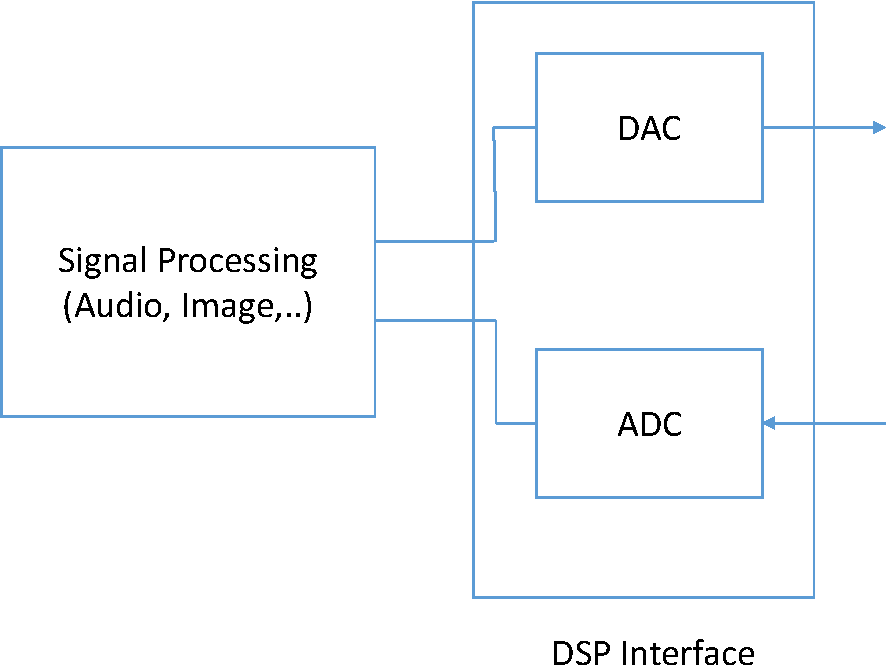
\includegraphics[width=0.4\textwidth]{dsp}
\end{figure}

\section{ADC Converter\label{sec:adc}}

An analog to digital converter is a system that converts an analog signal, such as sound picked up by a microphone, into a digital signal. There are several architectures of the ADC converter that can be implemented. Three different implementation method are mentioned here. However just one of them is going to be used.

\begin{itemize}
    \item \nameref{sec:vco-based-adc}
    \item \nameref{sec:binary-search}
    \item Using an external ADC chip like MPC3002
\end{itemize}

\subsection{VCO-based ADC\label{sec:vco-based-adc}}

The VCO-based ADC comprises a VCO and a frequency-to-digital converter (FDC) as shown in \fref{fig:vco-based-adc}. The VCO converts the input voltage into frequency information and the frequency-to-digital converter translates this frequency information into a binary code by integrating the VCO output over a time interval $T_s$. A simple frequency-to-digital converter is also shown in \fref{sec:vco-based-adc}, consists of a counter and a register. The counter counts the edges in the VCO output within the given time interval $T_s$ and stores the value in the register.

\begin{figure}
    \centering
    \caption{VCO-based ADC\label{fig:vco-based-adc}}
    \includegraphics[width=0.5\textwidth]{vco-graph}
    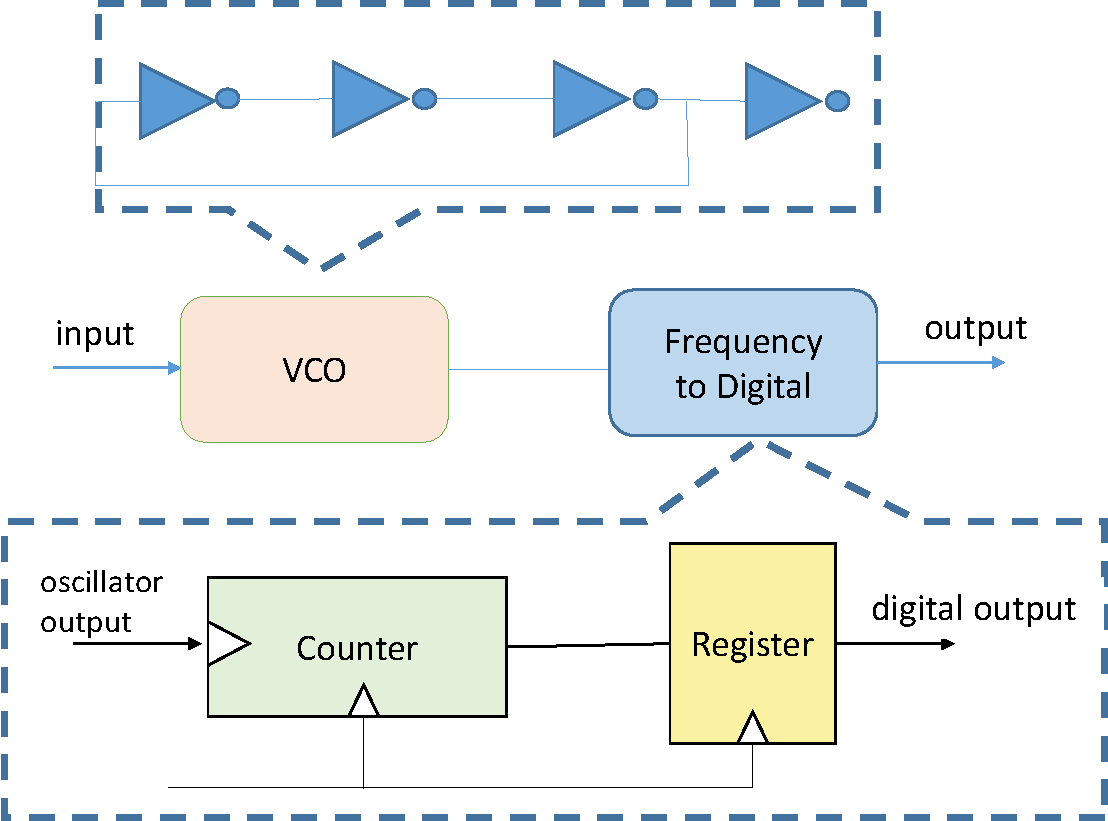
\includegraphics[width=0.6\textwidth]{vco}
\end{figure}

\subsection{Binary Search Algorithm\label{sec:binary-search}}

By using a digital comparator and comparing the two inputs and producing 1 or 0 for binary search module you will find the input value. Essentially, the strategy of all these converters is to put a value on the input of digital comparator, compare the value with the input voltage and then update the DAC for another guessed value. This is repeated until the sought value is obtained. The differences between the converters essentially lie in the guess-strategy or search algorithm.

\begin{figure}
    \centering
    \caption{Binary search module with a digital converter\label{fig:binary-search}}
    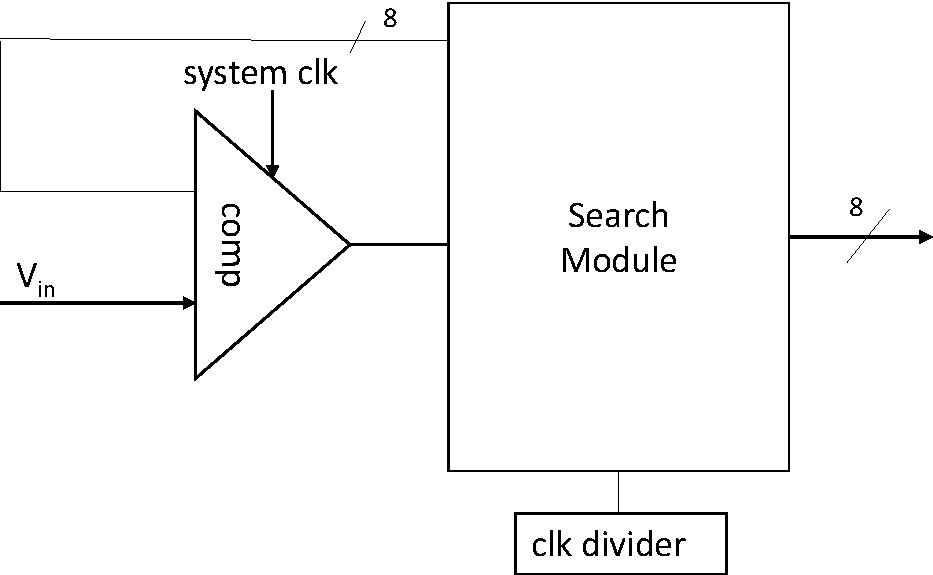
\includegraphics[width=0.4\textwidth]{bs}
\end{figure}

\subsubsection{Search Module}

A search algorithm is a method of locating a specific item of information in a larger collection of data.
In computer science, there are many methods to find the position of a particular value within an array.

The simplest search algorithm that comes to mind is linear search. This method uses a loop to sequentially step through an array, starting with the first element. It compares each element with the value being searched for and stops when the desired value is found or the end of the array is reached. Linear search is very simple to implement, and is practical when the array has only a few elements, or when the search is performed in an unordered list. However, this algorithm is slow. It takes time proportional to the number of item in the list to find the desired value. In other words, it is an $O(N)$ (order n) algorithm and is not cost-effective when we have large amount of data.

The more efficient algorithm to find an item when we have a sorted array is binary search. A binary search requires fewer comparisons than a linear search. In fact, it uses a \textit{divide and conquer} approach. This algorithm compares the median element in the sorted array to the desired input value in each step. If the input value is equal to the median value, then search is done. Otherwise, based on the comparison, it can eliminate half of the search space. If the input value is less than the middle element's value, then the algorithm repeats its action on the sub-array to the left of the middle element, or if the input value is greater, on the sub-array to the right. By doing this repeatedly, it will eventually be left with a search space consisting of a single element, i.e. the desired input value.

For example, consider the following sequence of integers sorted in ascending order and say we are looking for the number 43:
\begin{center}
\colorbox{Gray!10}{1\qquad 7\qquad 12\qquad 15\qquad 23\qquad \colorbox{Red}{\color{White}\bfseries 35}\qquad 43\qquad 49\qquad 52\qquad 57\qquad 61}
\end{center}
First, we compare 43 with the median value, which is 35 in this example. Since 43 is greater than 35, our search space is reduced to:
\begin{center}
\colorbox{Gray!10}{43\qquad 49\qquad \colorbox{Red}{\color{White}\bfseries 52}\qquad 57\qquad 61}
\end{center}
Again, we compare 43 with median value (52). This brings the search space reduce to:
\begin{center}
\colorbox{Gray!10}{\colorbox{Red}{\color{White}\bfseries 43}\qquad 49}
\end{center}

Depending on how we choose the median of an even number of elements, we will either find 43 in the next step or chop off 49 to get a search space of only one element. Either way, we will reach to the desired value in the sorted array.

The operation of ADC can be modeled as a search problem. In this problem, sensors' values that DAC is able to produce form the sorted array and input voltage is the element we search for. So, in case of our system, first, the total possible range of values is divided into two and the input voltage value is checked for presence in the upper half-space or the lower using the comparator ($>128$ or $<128$ for an 8-bit converter). If the comparator output indicates that the result is over the middle value, then the half space is sub-divided into two equal spaces and the value is compared to that. Depending on the result, the upper or lower quarter is divided and so on. The process terminates when the remaining space can not be subdivided, because it is only one bit wide.

The Verilog code for the binary search algorithm is provided to you in a file named \path{BS_ADC.v}. Test the ADC converter by running this code on the FPGA. Verify the design. You can even use the LEDs on the board to show the output. Also, you can use the other methods as alternatives.

\designverification{}

\section{A Simple Audio Loop Test}

In this part, you are going to make an audio in-out loop inside the FPGA. You will play an audio signal (any speech or music file) from your PC and hear it with your earphones. To do this, as described before, ADC and DAC converters are required. You have constructed a DAC circuit in the previous experiment. Use a 10-bit DAC based on Lab 3 and also the ADC of \fref{sec:adc} as the interfaces of your signal processor.

\begin{enumerate}
    \item Instantiate the DAC and ADC modules inside a top-level Verilog design as \fref{fig:loop}
    \item Inside the processor, use a hex-to-7segment code to display the value of converted digital values 
\end{enumerate}

\begin{figure}
    \centering
    \caption{An audio in-out loop\label{fig:loop}}
    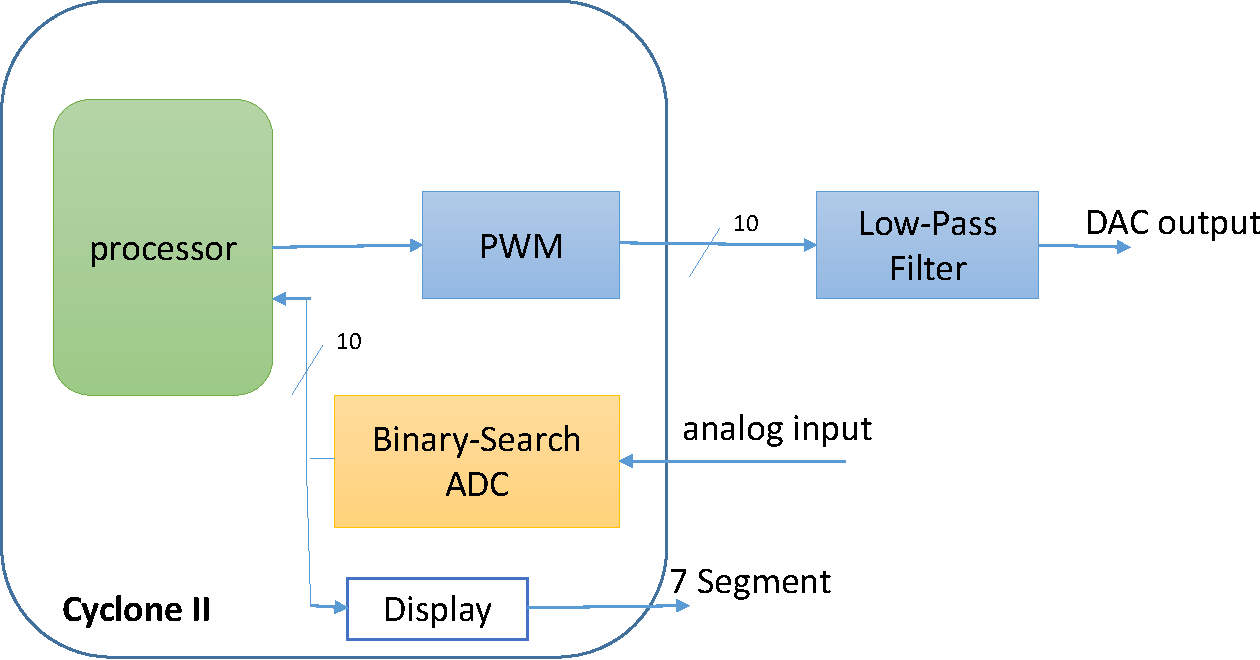
\includegraphics[width=0.6\textwidth]{loop}
\end{figure}

Use the frequency divider of the Experiment~1 that implements a ring oscillator as the source signal. In this case, the frequency selector of your function generator will be an external circuit. If you take this option, use dip switches to turn the parallel load inputs on and off.

\designverification{}

\section{FIFO\label{sec:fifo}}

In this part, you are going to learn about a memory structure called FIFO that stands for First Input First Output, a method for organizing and manipulating a data buffer, where the oldest (first) entry, or \textit{head} of the queue, is processed first. You can see the operation of a FIFO in \fref{fig:fifo}.
When a new data item arrives and the FIFO is not full, it is written to the FIFO. As a stored data item is retrieved, it is removed from the FIFO. If the buffer is full, it should not receive any more data; otherwise, existing store data would be corrupted. A \textit{full} status signal is asserted to tell the sender not send any more data. Similarly, an \textit{empty} status signal is used to indicate that the FIFO has no more data to provide. If the buffer is empty, it can not provide any data for retrieval.

\begin{figure}
    \centering
    \caption{Representation of a FIFO\label{fig:fifo}}
    \includegraphics[width=0.5\textwidth]{fifo}
\end{figure}

\Fref{fig:fifo-rtl} shows the RTL view of the FIFO. This memory structure has read and write pointers that keep track of data in FIFO. When the pointer gets the maximum ram depth, the signal \lstinline{full} gets 1 and when it reaches 0 the \lstinline{empty} signal gets 1.
According to this block diagram, the flow can be designed with four \lstinline{always} blocks as snippets~\ref{lst:write_pointer}, \ref{lst:read_pointer}, \ref{lst:read_data} and \ref{lst:status_counter}.
The \lstinline{write_pointer} \lstinline{always} block is for incrementing the pointer for writing data using \lstinline{wr} control signal. A similar procedure is true for the \lstinline{read_pointer} and \lstinline{read_data}.

The last block is used to control the \lstinline{full} and \lstinline{empty} signals. When the FIFO is reading and the reading has not finished yet, the counter must be decreased until it reaches zero. The same is true for writing and incrementing the counter hence it has not reached the maximum depth of RAM.

\begin{figure}
    \centering
    \caption{FIFO RTL view\label{fig:fifo-rtl}}
    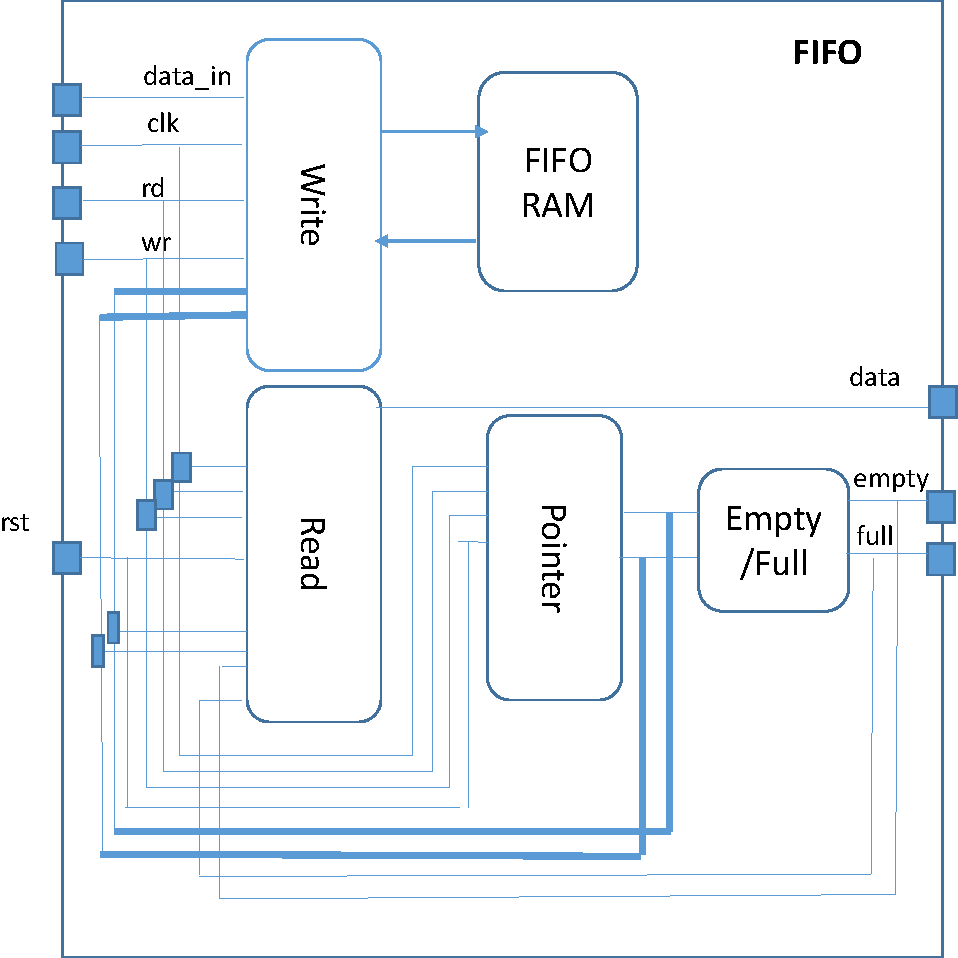
\includegraphics[width=0.7\textwidth]{fifo-rtl}
\end{figure}

\begin{multicols}{2}
\begin{lstlisting}[caption={\lstinline{write_pointer} \lstinline{always} block\label{lst:write_pointer}}]
always @(posedge clk or posedge rst)
begin: write_pointer
    if (rst)
    begin
        wr_pointer <= /* ... */;
    end
    else if (/* a control signal */)
    begin
        wr_pointer <= /* ... */;
    end
end
\end{lstlisting}
\vfill\null
\begin{lstlisting}[caption={\lstinline{read_pointer} \lstinline{always} block\label{lst:read_pointer}}]
always @(posedge clk or posedge rst)
begin: read_pointer
    if (rst)
    begin
        rd_pointer <= /* ... */;
    end
    else if (/* a control signal */)
    begin
        rd_pointer <= rd_pointer + 1;
    end
end
\end{lstlisting}
\end{multicols}

\begin{multicols}{2}
\begin{lstlisting}[caption={\lstinline{read_data} \lstinline{always} block\label{lst:read_data}}]
always @(posedge clk or posedge rst)
begin: read_data
    if (rst)
    begin
        data_out <= /* ... */;
    end
    else if (/* ... */)
    begin
        data_out <= /* ... */;
    end
end
\end{lstlisting}
~\\
\vfill\null
\begin{lstlisting}[caption={\lstinline{status_counter} \lstinline{always} block\label{lst:status_counter}}]
always @(posedge clk or posedge rst)
begin: status_counter
    if (rst) // read but no write
    begin
        status_cnt <= 0;
    end
    else if (/* ... */) // write but no read
    begin
        status_cnt <= /* ... */;
    end
    else if (/* ... */)
    begin
        status_cnt <= /* ... */;
    end
end
\end{lstlisting}
\end{multicols}

Complete the \lstinline{always} blocks based on the control signals and include them in a Verilog code for the FIFO.
For the ease of you, the RAM block code, named \path{RAM.v}, has been provided. Instantiate the RAM block and put all other required parts inside your code and make a project of it.
Test your design with a testbench and observe the results in ModelSim.

\designverification{}

\section{Producing Echo and Multiple Echo}

In this part of the experiment, you will design and test a circuit that simulates the effect of echo.
\Fref{fig:echo-concept} shows the components of a sound source reaching its listener:
the direct path signal $x(t)$ and
the echo signal $\beta x(t-T)$ which is weaker version of $x(t)$ attenuated by factor $\beta$, bounced off the floor. The echo signal is also delayed by $T$ relative to the direct-path signal $x(t)$.

\begin{figure}[b]
    \centering
    \caption{Concept of an audio echo\label{fig:echo-concept}}
    \includegraphics[width=0.5\textwidth]{echo-concept}
\end{figure}

\subsection{Simple Echo}

Based on \fref{sec:fifo} and the definition of FIFO, it is simple to apply such delay to an audio signal. This is illustrated in \fref{fig:simple-echo}.

\begin{figure}
    \centering
    \caption{Block diagram of a simple echo generator\label{fig:simple-echo}}
    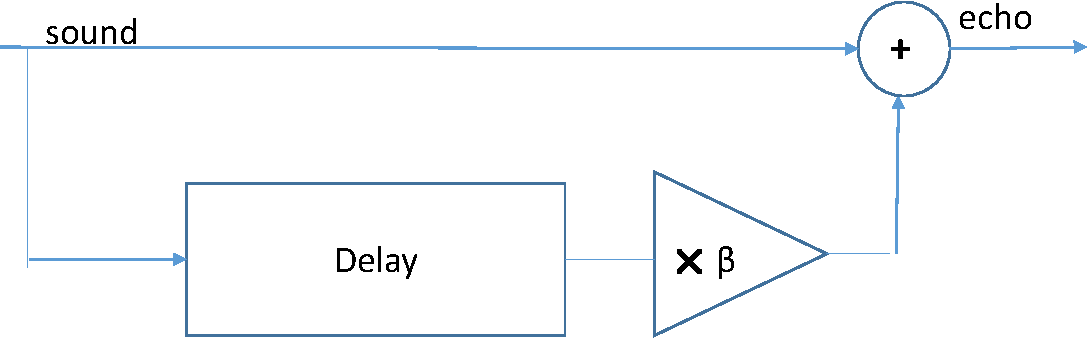
\includegraphics[width=0.5\textwidth]{simple-echo}
\end{figure}

Use the FIFO of \fref{sec:fifo} as a delay and a simple binary shift for the attenuation part. Design this echo generation system. 

\subsection{Multiple Echo}

In order to produce a multiple echo on an audio signal, it must be delayed and given feedback. Note that in this case the output is subtracted from the input.
\Fref{fig:multiple-echo} shows the block diagram of a multiple echo processor. A pulse generation block sends request for writing the sampled data in FIFO. The FIFO writes the input data and once it is full it starts reading from the FIFO. So one \lstinline{write_req} port will be enough for both operation. Based on this concept, guess the block with question mark. Use the FIFO of \fref{sec:fifo} and design the multiple echo system of \fref{fig:multiple-echo}. 

\begin{figure}
    \centering
    \caption{Block diagram of a multiple echo processor\label{fig:multiple-echo}}
    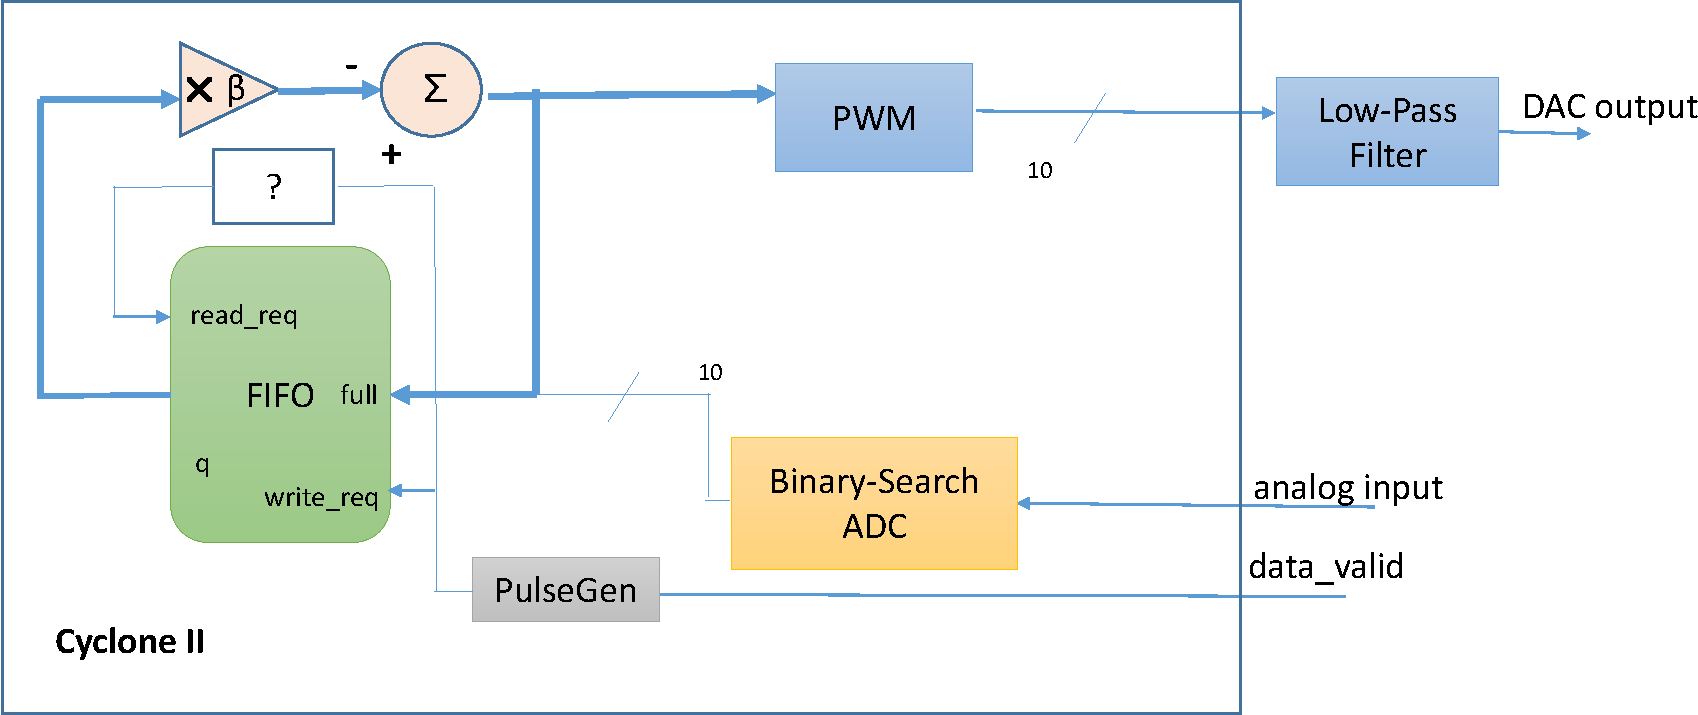
\includegraphics[width=0.7\textwidth]{multiple-echo}
\end{figure}

\designverification{}

\section*{Pre-Lab Assignment}
\addcontentsline{toc}{section}{Pre-Lab Assignment}
Before coming to the lab, answer these questions. The pre-lab needs to be handed in at the start of the lab.

\begin{enumerate}
    \item Complete the \lstinline{always} blocks \lstinline{write_pointer}, \lstinline{read_pointer}, \lstinline{read_data} and \lstinline{status_counter}.
    \item Write a testbench for the FIFO. Try to make a preliminary design at least.
\end{enumerate}


\section*{Acknowledgment}
\addcontentsline{toc}{section}{Acknowledgment}

This lab manual was prepared and developed by \href{mailto:ktbasharkhah@gmail.com?subject=[DLDLab]\%20}{Katayoon Basharkhah}, PHD student of Digital Systems at University of Tehran, under the supervision of professor Zain Navabi.

This manual has been edited by \href{mailto:hadi.safari@ut.ac.ir?subject=[DLDLab]\%20}{Hadi Safari}, undergraduate student of Computer Engineering at University of Tehran.

\end{document}
